\scanpage{73}
\mspage{72}
% E: drawing|lower left upper row|two vertices on a line and transverse rays
\figure{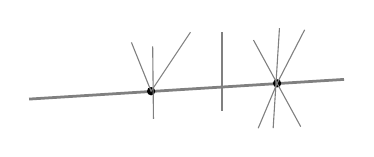
\begin{tikzpicture}[x=1cm,y=1cm]
\draw[gray,line width=1pt] (-2,0)--(2,.25);
\fill(-.45,.1)circle(1.5pt);\fill(1.15,.2)circle(1.5pt);
\draw[gray] (-.7,.72)--(-.45,.1)--(.05,.85);\draw[gray] (-.43,.67)--(-.42,-.25);
\draw[gray] (.45,-.15)--(.45,.85);
\draw[gray] (.85,.75)--(1.15,.2)--(1.45,-.35);\draw[gray] (1.5,.88)--(1.15,.2)--(.91,-.37);\draw[gray](1.18,.9)--(1.1,-.37);
\end{tikzpicture}}
% E: display|beneath two-vertex drawing written inverted|n-1 minus two terms
\[ (n-1)-(\unsure{\nu|\mu}-1)-(\unsure{\nu'|\mu'}-1) \qquad n-\nu \]
% E: drawing|lower middle upper row|two sloping parallel segments and dots
\figure{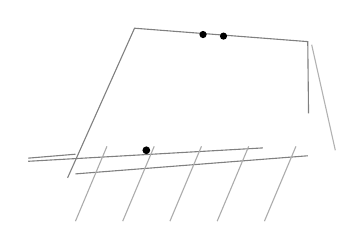
\begin{tikzpicture}[x=1cm,y=1cm]
\draw[gray] (-1.5,0)--(-.65,1.9)--(1.55,1.73)--(1.56,.82);
\draw[gray!60] (1.6,1.69)--(1.9,.35);
\draw[gray] (-1.4,.05)--(1.55,.28);\draw[gray](-2,.21)--(.98,.38);\draw[gray](-2,.25)--(-1.4,.3);
\fill(.22,1.82)circle(1.3pt);\fill(.48,1.8)circle(1.3pt);\fill(-.5,.35)circle(1.4pt);
\foreach \x in {-1.4,-.8,-.2,.4,1}{\draw[gray!65](\x+.4,.4)--(\x,-.55);}
\end{tikzpicture}}
% E: drawing|lower right upper row|point with six radial strokes
\figure{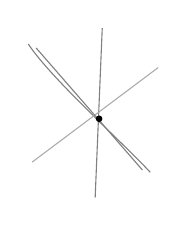
\begin{tikzpicture}[x=1cm,y=1cm]
\draw[gray](-.05,-1)--(.04,1.15);\draw[gray](-.9,.95)..controls(-.6,.5)and(.3,-.3)..(.65,-.68);\draw[gray!65](-.85,-.55)--(.75,.65);\draw[gray](-.8,.9)--(.55,-.65);\fill(0,0)circle(1.2pt);
\end{tikzpicture}}
% E: drawing|bottom left pencil construction|one vertex transverse line and arrow
\figure{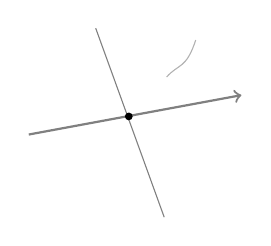
\begin{tikzpicture}[x=1cm,y=1cm]
\draw[gray,line width=.8pt,->](-1.4,-.15)--(1.3,.35);\draw[gray](-.55,1.2)--(.32,-1.2);\draw[gray!60](.72,1.05)..controls(.6,.68)and(.5,.75)..(.35,.58);\fill(-.13,.08)circle(1.4pt);
\end{tikzpicture}}
% E: drawing|bottom centre pencil construction|three crossing directions
\figure{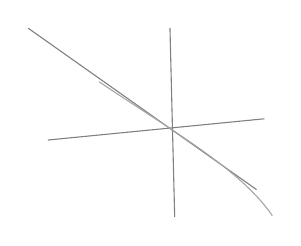
\begin{tikzpicture}[x=1cm,y=1cm]
\draw[gray](-1.55,-.12)--(1.2,.15);\draw[gray](0,1.3)--(.06,-1.1);\draw[gray](-1.8,1.3)--(1.1,-.75);\draw[gray!70](-.9,.62)..controls(.1,-.05)and(.9,-.5)..(1.3,-1.08);
\end{tikzpicture}}
% E: drawing|bottom centre right|polygon fan with doubled bent strip
\figure{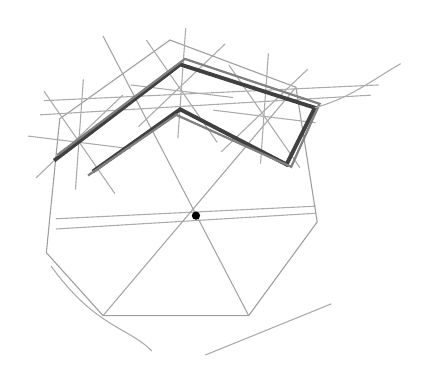
\begin{tikzpicture}[x=1cm,y=1cm]
\draw[gray!75] (-1.42,-.55)--(-1.25,1.15)--(.15,2.15)--(1.75,1.55)--(2.02,-.16)--(1.15,-1.35)--(-.7,-1.35)--cycle;
\draw[gray!65](-1.3,-.25)--(2,-.05);\draw[gray!65](-1.3,-.12)--(2,.04);
\draw[gray!70](-.7,-1.35)--(1.75,1.55);\draw[gray!70](1.15,-1.35)--(-.7,2.2);
\fill(.48,-.08)circle(1.5pt);
\draw[gray!65](-1.5,1.2)--(2.7,1.45);\draw[gray!65](-1.45,1.38)--(2.8,1.58);
\foreach \x/\y in {-1/.85,.3/1.5,1.35/1.18}{
\draw[gray!65](\x-.45,\y+.65)--(\x+.45,\y-.65);\draw[gray!65](\x-.55,\y-.45)--(\x+.55,\y+.6);\draw[gray!65](\x-.65,\y+.08)--(\x+.65,\y-.08);\draw[gray!65](\x+.05,\y+.8)--(\x-.05,\y-.6);
}
\draw[black!75,line width=1.4pt](-1.32,.62)--(.28,1.84)--(1.99,1.29)--(1.63,.57)--(.28,1.27)--(-.83,.48);
\draw[gray,line width=.8pt](-1.28,.69)--(.34,1.91)--(2.05,1.34)--(1.69,.54)--(.23,1.2)--(-.89,.43);
\draw[gray!65](1.99,1.29)..controls(2.45,1.42)and(2.7,1.63)..(3.08,1.85);
\draw[gray!65](-1.36,-.72)..controls(-.8,-1.5)and(-.37,-1.5)..(-.08,-1.8);\draw[gray!65](.6,-1.85)--(2.2,-1.2);
\end{tikzpicture}}
% E: text|bottom printed block inverted|JOB CRAY2
{\ttfamily
/*JOB=CRAY2,ACCT=*********,ALL=M06,MSGL=N\hfill J0424CNU\par
// JOB MSGLEVEL=(1,1),MSGCLASS=A\par
// EXEC PGM=IEFBR14\par}
% E: display|bottom manuscript inverted above sigma sequence|N=4n
\[N=4n\]
% E: display|bottom manuscript inverted first line|sigma0 sigma1 dash sigmaN-1
\[\sigma_0\sigma_1\mathbin{-}\sigma_{N-1}\ \big|\ \sigma_N=\sigma_0\qquad \sigma_i^2=1\]
% E: display|bottom manuscript inverted second line|rho1 sigma0 sigma1
\[\rho_1=\sigma_0\sigma_1\quad \rho_2=\sigma_1\sigma_2\quad\cdots\quad \rho_N=\sigma_{N-1}\sigma_N=\sigma_{N-1}\sigma_0\]
% E: text|bottom manuscript inverted right|rho_i squared one
$\rho_i^2=1$ i.e. deux $\sigma_i$ consécutifs (circulairement) commutent
% E: display|bottom manuscript inverted final line|rho1 rho2
\[\rho_1\rho_2=\sigma_0\sigma_2\qquad\rho_2\rho_3=\]
